\documentclass[10pt, letterpaper]{article}
\usepackage{graphicx}       % for inserting images
\usepackage{booktabs}       % for inserting tables
\usepackage{parskip}        % for formatting paragraphs
\usepackage{amsmath}        % for formatting math equations
\usepackage{array}          % for formatting tables
\usepackage{multirow}       % for formatting tables
\usepackage{wrapfig}        % for formatting wrap figures
\usepackage[font=small]{caption}    % for adjusting label size

\setlength{\parindent}{10pt}

\title{Application of Computer Vision and Robotic Arm in Cashew Nuts Production Line}
\author{Nam Tran, Minh Tran}
\date{TMA Solutions/RMIT University, Ho Chi Minh City, Vietnam} %November 25, 2022

\begin{document}

\maketitle

\begin{abstract}
    This paper proposes a novel method to automatize the quality control (QC) line of the cashew nut production process by implementing computer vision to self-detect faulted cashew nuts and have them removed automatically using a robotic manipulator. The machine vision is equipped with the Basler Ace 2 camera, allowing great compatibility with multiple computer vision applications at an industry level. With convolutional neural networks, the state-of-the-art pretrained algorithm – YOLOv4 – is implemented for real-time detection and classification of cashew nuts. The pick-and-place process to remove the defected cashew nuts is manipulated using a 4 DOF Parallel Robot (DeltaX), equipped with an external pneumatic logic control (PLC) system and a suction cup for picking the objects. The paper is expected to provide an automated solution to cashew nuts production and production lines in general, to further increase the efficiency and reduce the intense workload of the employees in factories.\par
    \textbf{Keywords}: Computer Vision, Deep Learning, Object Detection, Convolutional Neural Networks, Production Line, Robotic Manipulator, Cashew Nut, Delta-X, Pneumatic System.
\end{abstract}

\section{INTRODUCTION}
    Cashew is a popular agricultural product and plays a vital role in the export market worldwide. As a type of food, cashew nut offers many healthy benefits, such as cancer and cardiovascular prevention. It is also considered as a source of vitamin to protect the body against sideroblastic anemia and pellagra [1]. As the biggest cashew nuts exporter in the world, Vietnam has some of the largest cashew processing companies across many provinces, which requires a massive number of human resources. During the COVID-19 pandemic, most companies have been suffering from worker shortages, forcing them to cut down on many staffs. Moreover, the living condition and education of people living in developing areas have been significantly improved, which encourages many people to choose to work as white-collar worker, making the shortage of unskilled labor for many processing companies predictable.\par
    In recent years, automated solutions have been applied to cashew nuts production to aid humans in the industry. The grading and shelling machines are implemented to sort cashew nuts into different grades based on their sizes, shapes, colors, and perform operations to remove their shells [2, 3]. However, the automated systems were only applied to early stages of the production process, while in the final stage, human labors are still involved to examine quality of the nuts to be packaged and delivered. Because this job requires high concentration in a long period of time, workers tend to get exhausted, which leads to inaccuracy and inefficiency in production. Hence, this paper proposes an automated solution that aims to reduce the human workload during the final sorting process of a cashew kernel production line, by applying computer vision and parallel robot. The system should perform classification between a normal and a faulted cashew nut and automatically remove it from the production line.\par
    In general, the system is a combination of three significant modules: machine vision, the system processor (CPU), and robotics components, which include a robotic arm with a pneumatic system and conveyor belt controller. The machine vision system is responsible for providing a real-time camera stream, which will be fed into the system processor as the input for the detection function. The detection function relies on the state-of-the-art YOLOv4 detection algorithm to recognize the presence of defected cashew nut and record its respective coordinates. The coordinates will then be converted into robotic coordinates before being translated into the corresponding G-code, which commands the robotic arm to approach the desired position and remove the target.\par
    For computer vision system, YOLO employs convolutional neural networks (CNN) to provide real-time object detection with high speed and accuracy. This algorithm requires only a single forward propagation through a neural network to recognize the presence of the desired object, meaning that the prediction and detection are manipulated within 1 cycle [4]. The YOLO environments consist of many variants: Yolov1-v2-v3-v4-v5. The excellent learning capabilities allow YOLO to learn the representations of any target and utilize them for object detection. Furthermore, YOLO has its metadata file, where the pre-trained models can be obtained online with an impressive number of objects – up to 9000. Understanding the difficulties when the training process takes place on memory-constrained computers, a Lite version of YOLO was published later on [5], allowing even the portable device to successfully train the model without Graphics Processing Units (GPU). This great advantage helps to bring the YOLO approach to many developers that are willing to work with deep learning on neural networks and have their contributions to the application of the machine learning field. It is worth noted that regardless of longer training time, YOLO-series algorithms keep a good balance between speed and accuracy.\par
    For robotic manipulator system, DeltaX parallel robot is selected for our application. The robotic manipulator that has concurrent prismatic or rotary joints is defined as the parallel robot [6]. By applying the kinematics of 03 high-speed servo motors, the mechanism significantly enhances the processing speed for the Pick-And-Place application. Manipulated by the CPU controller, each motor handles the movement of an individual arm, thus the combination of all motors provides a synchronized motion among the X, Y, and Z axis. The main applications of delta robots are Shelf and Retail Ready Packing (picking and packing in logistic/ F\&B industries), and full layer packing. The advantages of the Delta robot are 30\% faster than the SCARA robot due to its mechanism, such as high speed and acceleration, high duty cycles. Moreover, the Delta robot also supports higher production rates because of its speed and its throughput. For safety purposes, the Delta robot is able to replace humans to do the high-speed and repetition processes, which usually cause stress injuries, fatigue, and lack of work satisfaction [7]. Another plus point of the Delta robot is saving space meaning that it can be mounted overhead, making them ideal for a small working environment.\par

\section{METHODOLOGY}
    In general, the project is a combination of three significant modules: the machine vision system, system processor (CPU), and robotic components, which includes the Delta robot with a pneumatic system and the conveyor belt controller.\par
    The machine vision system is responsible for providing a real-time camera stream, captured by Basler Ace camera. Then, the frames will be fed into the system processor as the input for the detection function. The detection process relies on the pre-trained YOLOv4 model with cashew nuts data, to recognize the presence of defected cashew nuts on the conveyor belt, track and record their respective coordinates. The coordinates will then be converted into robotic coordinates for the pick-and-place operation. From the recorded coordinates of the faulted cashew nuts, the corresponding G-code commands will be generated to control the DeltaX robot manipulator and the pneumatic system to approach and remove the target.\par

\subsection{System architecture}
In general, the project is a combination of three significant modules: the machine vision system, system processor (CPU), and robotic components, which includes the Delta robot with a pneumatic system and the conveyor belt controller.\par
The machine vision system is responsible for providing a real-time camera stream, captured by Basler Ace camera. Then, the frames will be fed into the system processor as the input for the detection function. The detection process relies on the pre-trained YOLOv4 model with cashew nuts data, to recognize the presence of defected cashew nuts on the conveyor belt, track and record their respective coordinates. The coordinates will then be converted into robotic coordinates for the pick-and-place operation. From the recorded coordinates of the faulted cashew nuts, the corresponding G-code commands will be generated to control the DeltaX robot manipulator and the pneumatic system to approach and remove the target.\par
\begin{figure}[h]
    \centering
    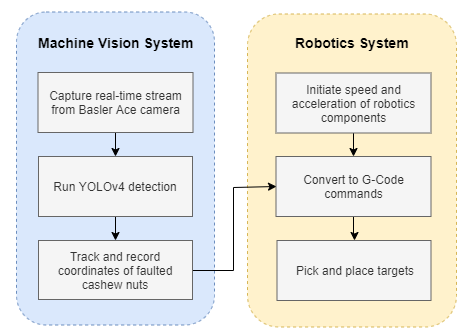
\includegraphics[width=0.8\textwidth]{fig1.PNG}
    \caption{General system structure diagram}
\end{figure}

\subsection{Detection and classification of cashew nuts}

\subsubsection*{Image acquisition}
    The dataset was collected by taking images of cashew nuts in two different conditions: normal and faulted nuts. Firstly, we prepared an amount of approximately 300 processed cashew nuts from the factory. Then, half of the batch was broken in half, either vertically or horizontally, to represent faulted cashew nuts, while others represent normal samples. After preparing a good number of samples, the nuts were placed on a conveyor belt, which will be used for the experiment later, and captured using an industrial camera installed on top of the samples (Figure 2).\par
    \begin{figure}[h]
        \centering
        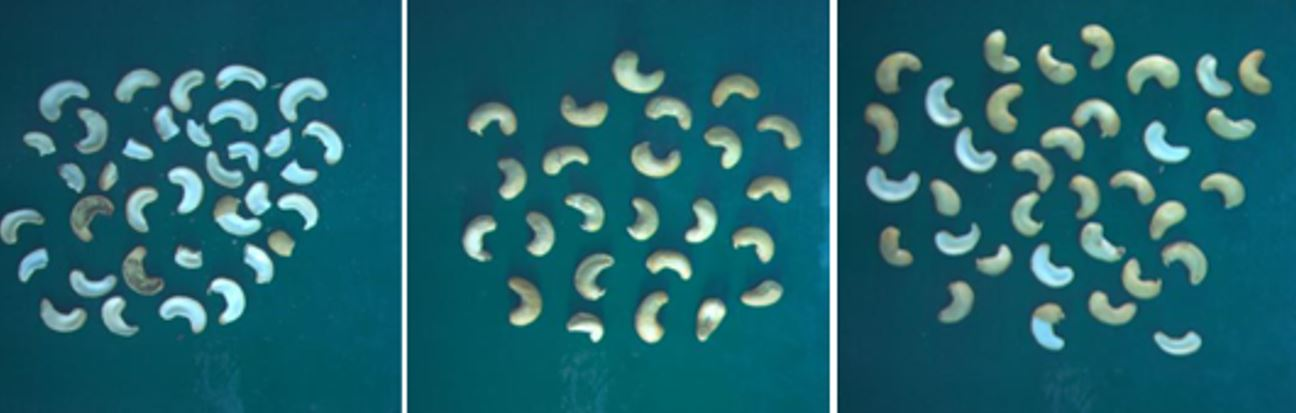
\includegraphics[width=0.9\textwidth]{fig2.JPG}
        \caption{Cashew nuts dataset faulted (left), standard (middle), mix (right)}
    \end{figure}
    The camera used in this project is the Basler Ace acA2040-25gc model, an area scan camera used for industrial purposes, equipped with a global shutter and the ams CMV4000 1’’ CMOS sensor. It can capture 25 FPS at 4 MP resolution (2046 x 2046 pixels). The camera was positioned 90o along the y-axis to capture the samples from a top-down view.\par
    \begin{figure}[h]
        \centering
        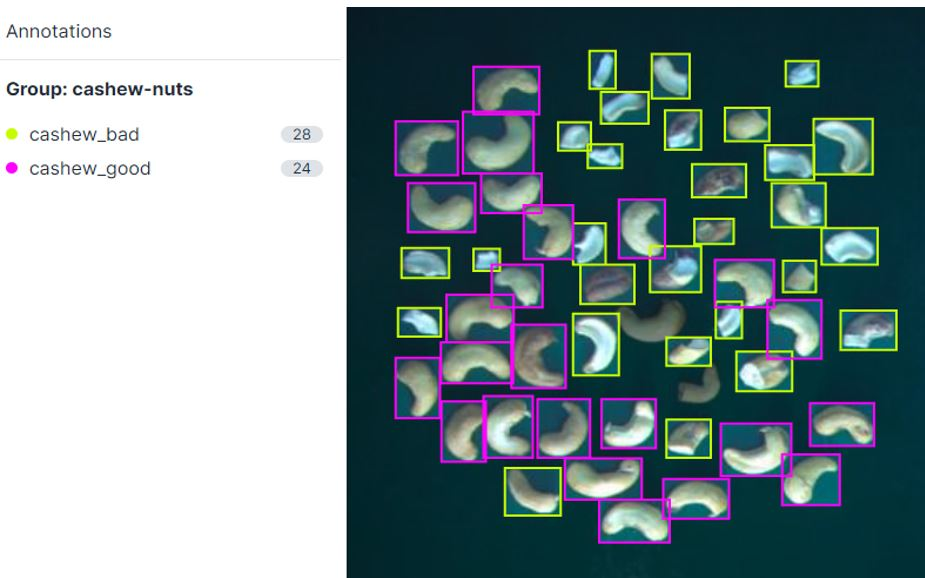
\includegraphics[width=0.8\textwidth]{fig3.JPG}
        \caption{Labelling process}
    \end{figure}
    After capturing 50 images, with an average of 30 cashew nuts in each image, including both normal and faulted objects, we have collected a total number of 1,500 samples. The images were then labeled manually by constructing bounding boxes around each object and classifying them into 2 classes: “cashew\_bad” and “cashew\_good”, representing faulted and standard cashew nuts, respectively (Figure 3).\par

\subsubsection*{Architecture design of YOLOv4 and YOLOv4-tiny}
    In this paper, the state-of-the-art YOLO (You Only Look Once) algorithm to train a model for the detection and classification of cashew nuts. This series of algorithms are proved to have a balanced ratio between speed and accuracy, which is suitable for real-time object detection applications.\par
    Different from two-stage object detection algorithms such as R-CNN or Faster R-CNN, which consists of a Region Proposal Network (RPN) to predict the possible bounding boxes, and a pooling stage to perform classification and bounding box regression; YOLO classifies and detects objects in a single stage, without the region proposal step [8].\par
    While two-stage object detectors give higher accuracy, they are relatively slow and not suitable for real-time purposes. However, one-stage detectors trade off some accuracy for higher inference speed, which is frequently adapted by a wider range of applications (traffic control, production lines).\par
    \begin{figure}[h]
        \centering
        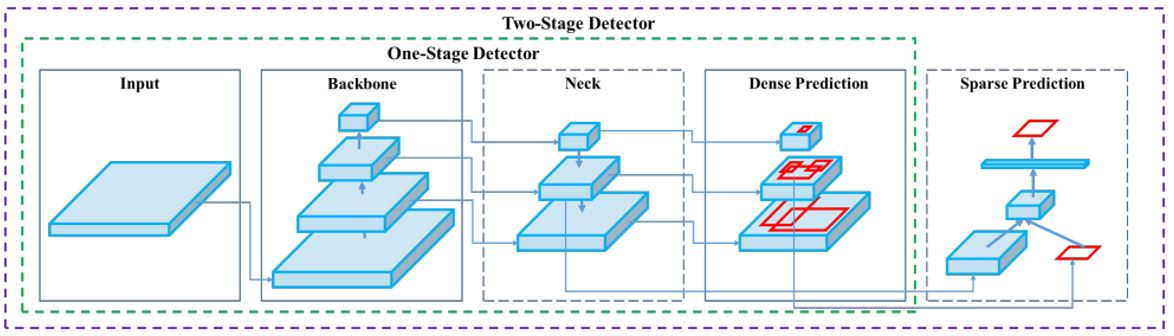
\includegraphics[width=\textwidth]{fig4.JPG}
        \caption{One-stage vs two-stage detector [8]}
    \end{figure}
    A one-stage object detector consists of 4 main parts: input, backbone, neck, and head. The input is a set of labeled images, or dataset, to be processed by the network; the backbone and neck are responsible for feature extraction and aggregation of the input dataset, and the head performs dense prediction to detect and classify the objects. From the official paper of YOLOv4 [9], to maximize the performance of the model, the choices for backbone, neck, and head are CSPDarknet53 [10], PANet [11] with additional SPP module, and YOLOv3 [9], respectively.\par
    \begin{figure}[h]
        \centering
        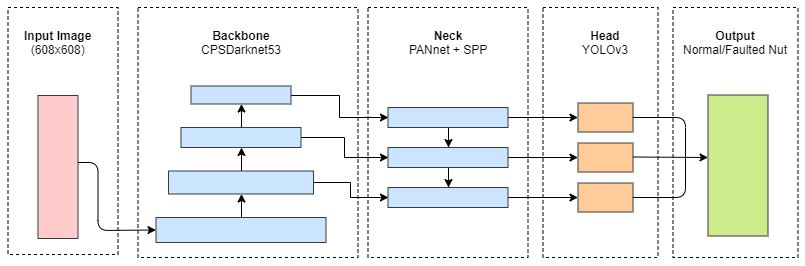
\includegraphics[width=\textwidth]{fig5.JPG}
        \caption{The architecture of YOLOv4}
    \end{figure}
    For achieving fast inference speed without the use of a graphics processing unit (GPU), YOLOv4-tiny was implemented in this project. YOLOv4 and YOLOv4-tiny have the same network structure, with CSPDarknet53 as the backbone, PANnet + SPP as the neck, and YOLOv3 as the head. However, the number of layers in the tiny version was greatly reduced, for instance, YOLOv4 has three YOLO heads and 137 pre-trained convolutional layers, while YOLOv4-tiny only has two heads and 29 convolutional layers [9]. Nonetheless, for simple 2-dimensional object detection applications, the detection accuracy compared to YOLOv4 is not significantly decreased, while the inference speed can be up to 8x faster.\par

\subsubsection*{Network configuration and model training}
    Prior to training the object detection model with the collected dataset, a Jupyter Notebook file is configured and run on a cloud-based platform - Google Colab - to utilize its GPU resources, thus, accelerate the training process.\par
    From [13], it is concluded that the performance of the object detection model can be improved by adjusting the input resolution of the dataset. Therefore, for this experiment, we will input different image dimensions in the YOLOv4-tiny network: 416 x 416, 608 x 608, 800 x 800, respectively; to evaluate the performance of the model. Furthermore, in order to avoid preparing a large dataset for training the model, we used transfer learning method, where a pre-trained and fine-tuned YOLOv4-tiny model was implemented. The model was pre-trained on MS COCO dataset, which includes 80 classes, 1.5 million samples, and 330,000 images [14]. By applying transfer learning, most of the feature maps from the pre-trained model can be reused and transferred to the new model, which will be trained further with the new dataset [13]. Before initiating the training process, the dataset of 50 images is randomly divided into three parts: 75\% for training, 15\% for validation and 10\% for testing.\par
    The main parameters initially set in the configuration of YOLOv4-tiny-416 (image resolution of 416 x 416), including layers number and type, number of filters, size and stride, and input and output tensors in the neural network, are listed in Appendix 1.\par

\subsubsection*{Evaluation methods}
    After training, the performance of the model can be evaluated by assessing the precision, recall, and F1-score. In the validation set, for each predicted bounding box i, it is compared with the ground truth and marked as true positive (TP) if the intersection over union \(IoU_i>IoU_{target}\), meaning the target is correctly detected [15]. Otherwise, if \(IoU_i < IoU_{target}\), or the target is not predicted, it will be defined as a false positive (FP). Finally, if the object is predicted incorrectly (wrong class), it is marked as a false negative (FN). The precision, recall, and F1-score are calculated based on the following equations.\par
    \begin{equation} \label{eq1} precision = \frac{TP}{TP + FP} \end{equation}
    \begin{equation} \label{eq2} recall = \frac{TP}{TP + FN} \end{equation}
    \begin{equation} \label{eq3} F1-score = \frac{2 \times precision \times recall}{precision + recall} \end{equation}
    Additionally, after calculating the above parameters, we compute the average precision (AP) as the area under the curve of precision over recall, which is a number between 0 and 1, at an IoU of 50\% [13]. \par
    The mean average precision (mAP) is later calculated by taking the average AP of each class, where N is the number of classes, and i is the class index.\par
    \begin{equation} \label{eq4} AP = \int_{0}^{1} p(r)\,dr \end{equation}
    \begin{equation} \label{eq5} mAP = \frac{1}{N} \sum_{i=1}^{N} AP_i \end{equation}

\subsection{Machine vision system}

\subsubsection*{Camera calibration}
    \begin{wrapfigure}{r}{0.3\textwidth}
        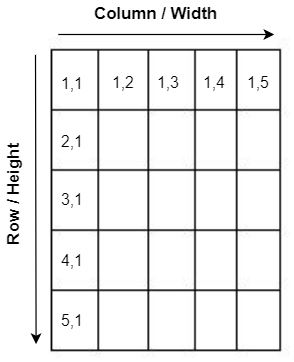
\includegraphics[width=\linewidth]{fig6.JPG} 
        \caption{Image represented as matrix}
        \label{fig6:wrapfig}
    \end{wrapfigure}    
    Following the camera setup process mentioned in the image acquisition section, where the Basler Ace is positioned on top of the conveyor belt, the next step for further integration with the whole system is to identify the position of each detected object.\par
    An image is made of multiple pixels (picture elements), and each pixel is a combination of RGB (red-green-blue) values. Therefore, a digital image can mathematically be represented as a 3-dimensional matrix, where each pixel is an element in the matrix. Similar to a matrix, the coordinate system of an image starts from the top left corner, its x-axis and y-axis move from left to right and top to bottom, respectively (Figure 6). A pixel presented on the image will have x and y coordinates, which are the number of columns and rows located in the matrix.\par
    Apply the same methodology to the computer vision system, as a faulted cashew nut is detected, its centroid will be marked and analyzed to locate the pixel coordinate on the image. Then, an operation of converting camera pixel coordinates to real-world coordinates needs to be done for further integration with the whole system. Due to our camera setup and the distortion prevention feature of Basler Ace’s camera lens, the conveyor belt presented on the camera frame is relatively flat, which makes the scene 2-dimensional.\par
    The goal of this calibration process is to determine the size of a pixel in the real-life unit (cm, mm, etc.). To achieve that, two main parameters are required, which are the height (or width) of the camera’s field of view (FOV) in pixel unit and real-life unit. With the known parameters, the height of a pixel in world coordinates can be calculated by taking the division of height in world coordinates, over the height in pixel coordinates. Height in world coordinates can be acquired by manually measuring how much frame height the camera can capture in a real-life unit. The simplest method is to place a measuring tool (ruler, caliper, measuring tape, etc.) under the camera’s FOV and then record the values. As for the height in pixel coordinates, it is the number of pixels along the y-axis or the number of rows in the matrix that represents the image. Since pixels are square-shaped, either width (x-axis) or height (y-axis) can be used for the conversion.\par
    The following equation shows the calculation of a pixel in world coordinates \par
    \begin{equation} \label{eq6} pixel\:length = \frac{height\:(or\:width)\:in\:world\:coordinates}{number\:of\:rows\:(or\:columns)} \end{equation}
    Then, to convert a pixel coordinate into the world coordinate, the coordinate (both x and y) on an image is multiplied by the previously calculated pixel length in the real-life unit.\par
    \begin{equation} \label{eq7} x_{world} = x_{pixel} \times pixel\:length \end{equation}
    \begin{equation} \label{eq8} y_{world} = y_{pixel} \times pixel\:length \end{equation}
    
    For this project, since measuring the height of the camera frame with a ruler possesses inaccuracies after several experiments, we decided to use white paper and place it on the conveyor belt, right underneath the camera, then measure the width and height of the paper manually (Figure 7). The paper has a height of 297 mm and a width of 210 mm (the size of a standard A4 paper). Then, adopting the selectROI function from OpenCV, a rectangle box is constructed around the A4 paper, and the camera frame is cropped to only capture the newly selected region of interest (ROI). After acquiring a new FOV, height and width in world coordinates would be equal to the A4 papers. To be compatible with the screen resolution, the camera frame height is resized to 800 pixels.\par       
    \begin{figure}[h]
        \centering
        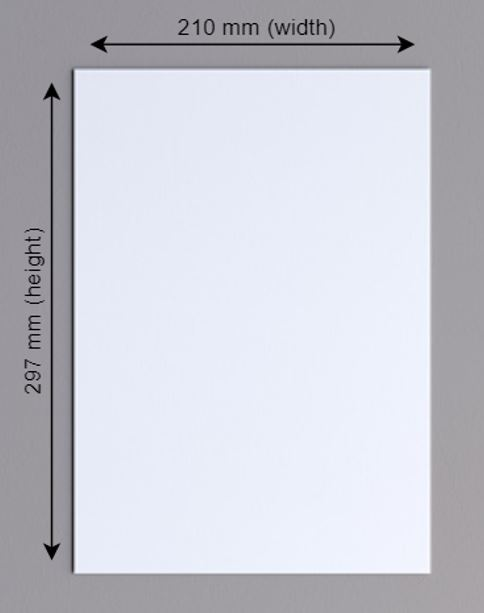
\includegraphics[width=0.4\textwidth]{fig7.JPG}
        \caption{Height and width of ROI}
    \end{figure}
    Knowing the height in world coordinates of 297 mm and pixel coordinates of 800 px, we can find the length of one pixel:\par
    \begin{equation} \label{eq9} pixel\:length = \frac{297\:mm}{800\:px} = 0.37\:mm/px \end{equation}
    By multiplying each detected target’s centroid with 0.37, we can find the (x, y) coordinate of that object in millimeters. \par

\subsubsection*{Detection process}
    After ensuring the camera has been connected and the meta-data file or pre-trained YOLOv4 is loaded successfully, the detection can be initiated. The system will receive and check the existence of the target by each frame. The “confidence” value of the detection algorithm can be adjusted to determine the accuracy of the detection process. When the target is identified, it will be assigned by a value, together with a red bounding-box wrapped outside. The algorithm also calculates the coordinates of the target, which is vital for the tracking process. To keep track of the target within multiple frames, the Non-Max Suppression (NMS) algorithm is utilized to merge multiple nearby bounding boxes of a single target in multiple frames into a single bounding box.\par
    \begin{figure}[h]
        \centering
        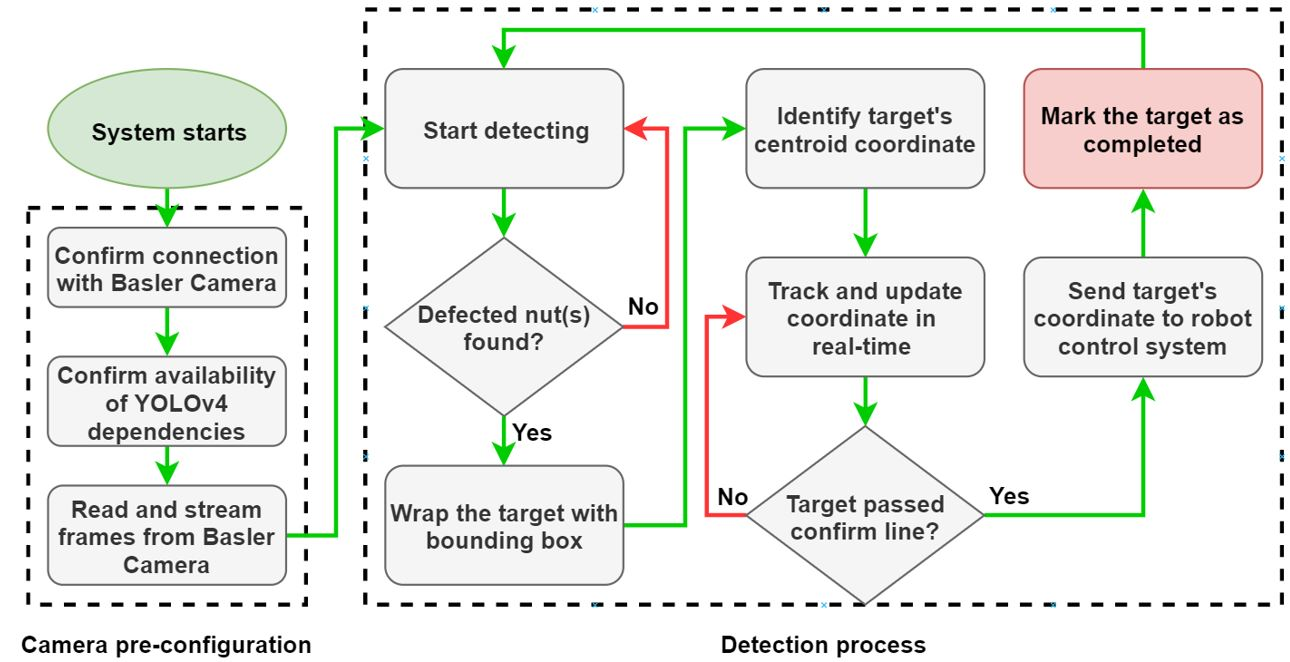
\includegraphics[width=\textwidth]{fig8.JPG}
        \caption{Workflow of camera and detection module}
    \end{figure}
    A border line (or confirm line) will be used to determine when to send the target coordinates to the robotic system. When the defected cashew crossed the line, its coordinate will be saved and sent to a “storage”, which will be used later by the robotic system. To prevent the system from continuously sending the coordinate of a single target, the target’s ID will be recorded when the system successfully sent the coordinate and marks the target as completed.\par

\subsection{DeltaX robot manipulator}

\subsubsection*{Robot arm configuration}
    \begin{table}[h!]
        \caption{Configuration of Delta XS D800 (Deltaxstore.com)}\label{table1}
        \centering
        \renewcommand{\arraystretch}{1.5}
        \begin{tabular}{l l l}
            \hline
            Unit & Value & Working space \\ \hline
            \begin{minipage}{4.3cm}
                Payload (kg) \\\\ Reach (mm) \\\\ Repitition accuracy (mm) \\\\ Position accuracy (mm)
            \end{minipage}
            &
            \begin{minipage}{3cm}
                $2\:kg$ \\\\ $800\:mm (diameter)$ \\\\ $\pm\,0.15\:mm$ \\\\ $0.2\:mm$
            \end{minipage}
            &
            \begin{minipage}{0.3\textwidth}
                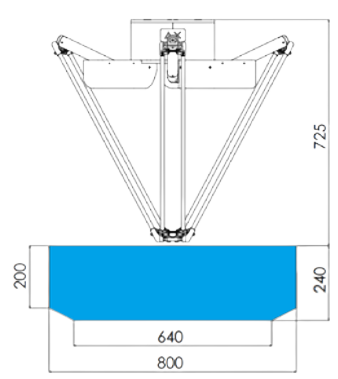
\includegraphics[width=\linewidth, height=40mm]{DX.png}
            \end{minipage}
            \\ \hline
        \end{tabular}
    \end{table}
    The Delta XS D800 parallel robot configuration shown in Table 1 is the current common configuration of the robot which is appropriate to the requirements of this application such as high flexibility, high accuracy, low payload, and saving space.\par
    Regarding the table above, the structure of the robot is concurrent with both prismatic and rotary joints. It is designed for overhead mounted machines with 3 motors placed in the base structure which directly connect to three leading arms driving three appropriate force arms below. The advantage of this robot type is reducing the weight within the arms which provides very high acceleration and speed capability [16]. The limitation of this robot is its low payload capacity, and the maximum payload of the applied robot in this application is 2 kg. In the next part, the pneumatic system design will be presented.\par

\subsubsection*{Pneumatic system}
    The pneumatic system is integrated with a robotic manipulator to create the mechanism of a vacuum to pick the faulty cashew nuts. The diagram of the system design is shown in Figure 9.\par
    There are five main parts in the pneumatic system including an air compressor, air preparation unit (FR), control valve, ejector, and suction cup. Firstly, the air compressor supplies air to the system with a pressure of 6 bar and 200L/min of air flow. These compressed air travel through the tube to the next component known as air preparation unit FR which stands for Filter and Regulator. This unit separates the water and dust of the air flow, and the regulator is applied to adjust the air pressure supplied to the system. The next step is to direct it through a directional valve control which is operated by the digital signal as controlled by PLC. Then, the airflow goes through the ejector to be changed from the pushing force to the vacuuming feature. Finally, the last component approaching picked objects is 2.5 bellows suction cup. The holing force of the pneumatic system is 1.56 N.\par
    \begin{figure}[h]
        \centering
        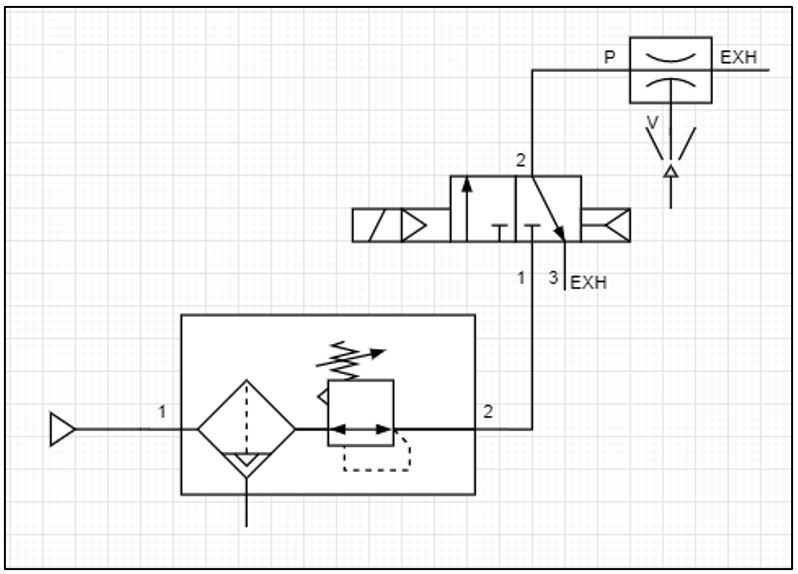
\includegraphics[width=0.6\textwidth]{fig9.JPG}
        \caption{Pneumatic System Diagram}
    \end{figure}

\subsubsection*{Elements of the robot controller}
    DeltaX robot is produced to have the same working mechanism as a CNC machine, thus, it works by receiving external G-code commands sent to the serial port and can be entirely controlled by a PC. The figure below illustrates the machine controller unit of DeltaX.\par
    \begin{figure}[h]
        \centering
        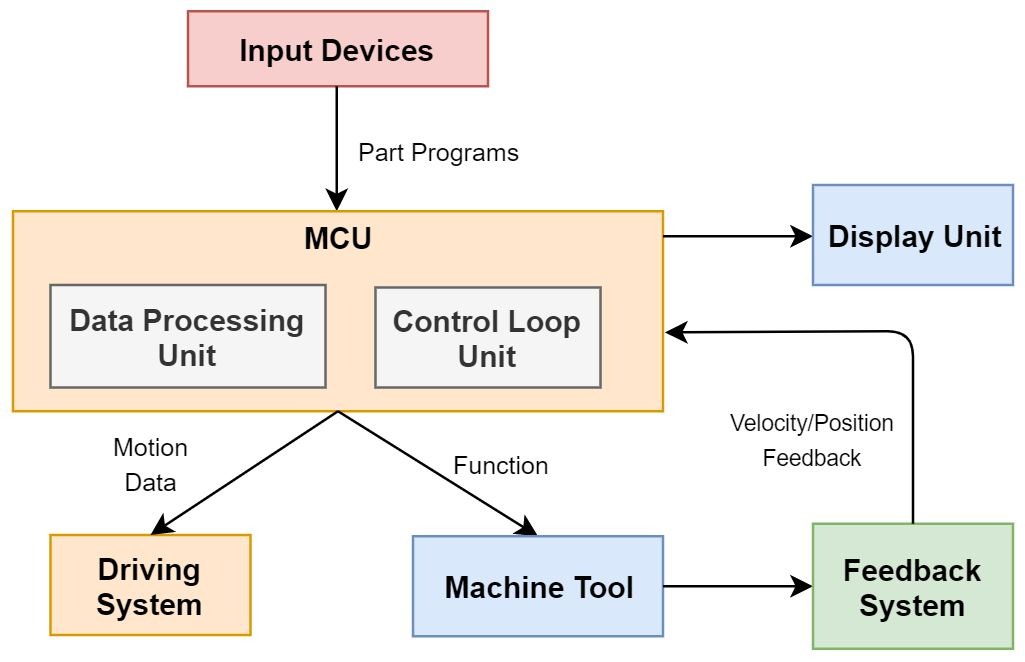
\includegraphics[width=0.7\textwidth]{fig10.JPG}
        \caption{Block diagram of the robot controller box}
    \end{figure}
    To operate any movement of the robot, the G-code command is sent from the PC to the robot MCU (Teensy Duino) by using TTL Serial (UART transmission). Then, the optimized firmware in Teensy Duino interprets, translates, and executes the sequence of the program to operate the motor drive (HB808C hybrid servo driver), which will drive the Hybrid Servo 57HSE to move the arm. For each hybrid Servo motor, its encoder will send the position feedback and velocity feedback to the MCU to create a close loop system.\par

\subsubsection*{Power supply unit}
    The power source of 24V-20A is the power supply for the whole system. The input voltage range of this AC to DC voltage converter is 110-220V AC and the output is 24V DC with ± 0.1V precision. The output current for the power supply is 15A without adjustment.\par

\subsubsection*{MCU Teensy Duino}
    The Teensy 4.0 board is dependent on the high-performance ARM Cortex M7 processor which operates at a maximum frequency of 600 MHz, ARM Cortex M7 processor. It has an extensive range of 24 I/Os pins with 40 digital pins. The number of analog pins and the PWM pins of Teensy is 14 pins and 27 pins which are approximately twice more than the Arduino, and this is the advantage of using Teensy to control many motors at the same time and save space due to its small size [17].\par

\subsubsection*{Motor drive}
    HSS57 is a hybrid stepper servo motor driver with 2 phases nema 23 series. This model adopts a new generation 32-bit DSP with the vector control technique which prevents the losing step of the stepper motor and ensures the precision of the motor. At the higher speed, the torque reduction is much lower than the stepper motor with the open loop. HSS57 also supports the channel of the encoder for the close loop system which is an ideal enhancement to develop the accuracy of the system compared to the open loop system.\par

\subsubsection*{Hybrid servo motor}
    The Hybrid servo motor 57HSE is a two phases stepper motor with encoder feedback which is designed to work with the HSS57 motor driver to create a hybrid close loop system (no more loss of step). The coils inside are 100\% pure cooper wires with low current consumption, low-temperature rise, high efficiency, and long lifetime. The final perfect geared motor can be produced by high efficiency and extreme performance motor cooperates with the accuracy and reliable gears [18].\par

\subsection{Cashew nuts picking strategy}

\subsubsection*{Robot operation to pick and place a nut}
    To begin with, the PC will send the command “G28” to send the robot back to the HOME position (Figure 12). At the same time, the values of velocity, acceleration, and jerk will also be set by sending the command “M210 F500 A10000 J1000000”.  After receiving the coordinates of the nut from the camera, these coordinates are put into a function to update the coordinates of that faulted nut every 0.1 second. The updated displacement of the nut on the linear conveyor depends on the conveyor constant speed \(v_belt\) and the updated time \(t_update\). Since the coordinate of a nut only changes along the conveyor in the Y axis while the X element is kept the same, the following formula is applied to calculate the current position of a nut.\par
    \begin{equation} \label{eq10} x_{current} = x_{initial} \end{equation}
    \begin{equation} \label{eq11} y_{current} = y_{last} - (t_{update} \times v_{belt}) \end{equation}
    As moving closer to the original point of the robot, the Y coordinate of the nut is decreased because the moving direction of the nut is inverted to the positive direction of the system and whenever the value \(Y_current\) of any nut is lower than 300 mm, the vacuum will be turned on by receiving command ‘’M03 D01’’ and the robot will move to picking position by commanding “G01 X[value] Y[value] Z[value]” to pick the nut and go back to drop off position. Finally, sending “M05 D01” to deactivate the vacuum to release the nut.\par
    \begin{figure}[h]
        \centering
        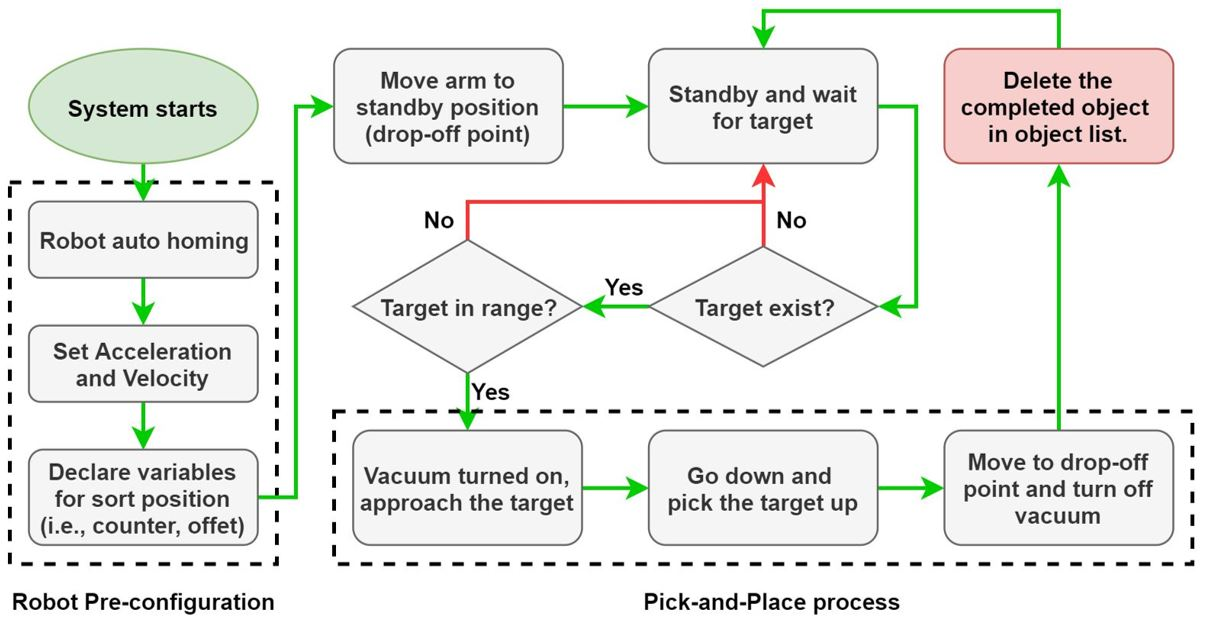
\includegraphics[width=\textwidth]{fig11.JPG}
        \caption{Pick and place workflow diagram}
    \end{figure}
    The challenges of this method are that firstly it depends on the accuracy of the nut initial position. This means the object detection system has to define precisely the initial position of the nut. If it is not formed and precise, the real-time updated position of the nut while moving on the conveyor is impacted. The second factor that can affect the current position of a nut is the constant speed of the conveyor. The actual running speed of the conveyor has to be constant as the value set to it at the start.\par

\subsubsection*{Reference frame and frame transformation}
    The most important part of the system is to select suitable reference frames. The robot (R), the camera (C), and the conveyor belt (B) reference frames are described in Figure 12. In the camera frame, the cashew nut is defined as a point P since the orientation of the nut is not involved in this application. To define the faulty nut position concerning the Delta robot frame, the rotational transformation matrix is defined based on the schematic below\par
    \begin{figure}[h]
        \centering
        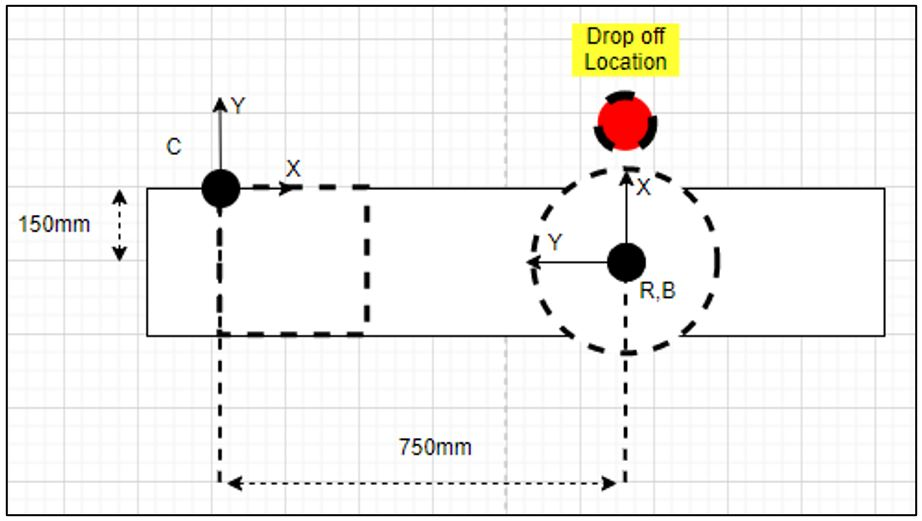
\includegraphics[width=0.65\textwidth]{fig12.JPG}
        \caption{The work cell layout with the reference frames}
    \end{figure}
    Since we only focus on 2-dimension horizontal plane, the 2x2 transformation matrix \(T_{i,j}\) depicts the i-th reference frame with respect to the j-th frame. In this case, this matrix can be obtained by the following transformation matrices: ${}^{R}_{C}R$ is the rotational matrix between camera and robot around z-axis, ${}^{C}P$ are the coordinates of nut in the camera frame, ${}^{R}ORG_{cam}$  is the translation matrix of the origin of the camera frame to the robot frame. The matrices are illustrated as follows\par
    \begin{equation} \label{eq12} 
        {}^{R}_{C}R = 
        \begin{bmatrix}
            \cos{\theta} & -\sin{\theta}\\
            \sin{\theta} & \cos{\theta}
        \end{bmatrix}
        =
        \begin{bmatrix}
            0 & -1\\
            1 & 0
        \end{bmatrix}_{\theta = 90^{\circ}}
    \end{equation}

    \begin{equation} \label{eq13} 
        {}^{R}ORG_{cam} = 
        \begin{bmatrix}
            150\\750
        \end{bmatrix}
    \end{equation}

    \begin{equation} \label{eq14} 
        {}^{C}P = 
        \begin{bmatrix}
            x_{initial}\\y_{initial}
        \end{bmatrix}
    \end{equation}
    This is the mapping problem involving both translation and rotation, therefore, the position of the target in the robot frame is defined as\par
    \begin{equation} \label{eq15} 
        T_{C,R} = {}^{R}_{C}R \times {}^{C}P = 
        \begin{bmatrix}
            x_{initial}\\y_{initial}
        \end{bmatrix}
        + {}^{R}ORG_{cam}
    \end{equation}

    \begin{equation} \label{eq16} R
        \begin{bmatrix}
            x_{initial}\\y_{initial}
        \end{bmatrix}
        =
        \begin{bmatrix}
            0 & 1\\
            -1 & 0
        \end{bmatrix}_{\theta = 90^{\circ}}
        \times {}^{C}
        \begin{bmatrix}
            x_{initial}\\y_{initial}
        \end{bmatrix}
        +
        \begin{bmatrix}
            150\\750
        \end{bmatrix}
    \end{equation}
    As a result, the positions of the camera, conveyor, and robot must be set up and calibrated deliberately to ensure that the targets’ coordinates are precise during the running time of the system.\par

\subsubsection*{Picking position prediction formula}
    After the coordinates of a target nut are sent to the robot, the pick-and-place (PNP) process is illustrated in this section. The PNP process for the proposed system consists of two main movements: a movement from the drop-off location to the picking location, and a movement from the picking point back to the drop-off point.\par
    Because the positions of the moving targets change over time, the first movement is dynamic. Since the picking nut is moving on the conveyor at a constant speed, the picking and placing prediction algorithm has been presented to approximately define the position that the end effector of the robot will arrive to pick the moving object. Figure 13 shows the position of robot end-effector ee and the position of nut P at time t as the prediction algorithm defines the movement from the drop-off location (starting point) to the picking-up position (ending point).\par
    \begin{figure}[h]
        \centering
        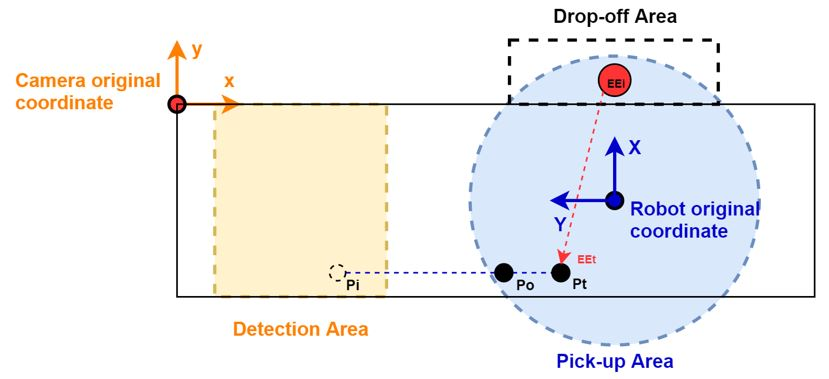
\includegraphics[width=0.75\textwidth]{fig13.JPG}
        \caption{The part position prediction diagram}
    \end{figure}
    To be specific, at the moment the nut goes into the picking area of the robot, the robotics system identifies the picking point where the moving nut and the robot will contact on the conveyor. The method applied to figure out the robot movement formula from point to point is the S curve. This means that from a drop-off point, the robot is accelerated to a constant velocity, and then it is decelerated as the final acceleration and velocity are zero when the robot arrives at the required destination.\par
    A full S-curve motion consists of 7 phases (Appendix 2). In Phase 1, the robot starts from the rest and linearly accelerates until it reaches the maximum acceleration. In Phase 2, the robot keeps its maximum acceleration until it has to decelerate as approaching the maximum velocity. This happens in Phase 3 as the acceleration starts to linearly decline until it goes down to zero. In Phase 4, until the deceleration happens, the control velocity is constant. At this point, the acceleration of the robot decreases in a manner symmetric to Phases 1, 2, and 3 [19]. The below formula is an S-curve equation in the continuous form.\par
    \begin{equation} \label{eq17} P_T = V_o + V_o{T} + \frac{1}{2} A_o{T^2} + \frac{1}{6} JT^3 \end{equation}
    \begin{equation} \label{eq18} V_T = V_o + A_o{T} + \frac{1}{2} JT^2 \end{equation}
    \begin{equation} \label{eq19} A_T = A_o + JT \end{equation}
    where:\\
    $P_o,\:V_o,\:A_o$ are starting position, velocity, and acceleration of robot\\
    $P_T,\:V_T,\:A_T$ are posotion, velocity, and acceleration of robot at time T\\
    $J$ is jerk
    \par
    According to the above three fundamental equations, the formulas for jerk, acceleration, velocity, and position of the robot in each phase are shown in the table (Appendix 3). From these motion parameters equations, the derived formula for the position of the robot is built and shown below, with the unknow variable $t$. \par
    \begin{equation} \label{eq20} P_{robot} = P_6 + v_6(t-t_6) + \frac{1}{2} a_6(t-t_6)^2 + \frac{1}{6} J(t-t_6)^3 \end{equation}
    Besides, the velocity of the conveyor is constant so the position formula of moving nut respect to time is shown below\par
    \begin{equation} \label{eq21} P_{nut}(t) = P_{{o}_{nut}} - tV_{conveyor} \end{equation}
    To define the time \(t_c\) and point \(P_T\) that the faulty nut and the robot will meet on the conveyor, we must set the formula and then solving for the unknow time \(t_c (s)\)\par
    \begin{equation} \label{eq22} P_{robot}(t) = P_{nut}(t) \end{equation}
    \begin{equation} \label{eq23} P_6 + v_6(t-t_6) + \frac{1}{2} a_6(t-t_6)^2 + \frac{1}{6} J(t-t_6)^3 = P_{{o}_{nut}} - tV_{conveyor} \end{equation}
    Finally, the picking position is defined as\par
    \begin{equation} \label{eq24} P_{picking} = P_T = P_{{o}_{nut}} - tV_{conveyor} \end{equation}
    As a result, with the inputs of the initial position of the robot end effector and the cashew nut, the picking position prediction formula can define the position and time that the end effector and the robot will meet each other. This formula is applied to a single nut and the next section will discuss how the robotic manipulator deals with multiple nuts.\par

\subsubsection*{Picking order arrangements for a series of nut}
    In the object detection area, the camera will define a series of faulty nuts which need to be removed. The challenge is deciding to figure out which nut should be picked first. Because the picking area of the robot is a circle as shown below, the applied method is to calculate the time each nut takes to reach the circle, and then the picking order will be decided depending on this time.\par
    \begin{figure}[h]
        \centering
        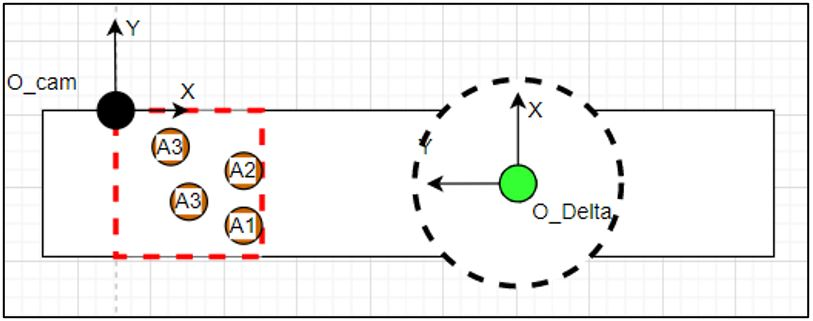
\includegraphics[width=0.65\textwidth]{fig14.JPG}
        \caption{Picking multiple nuts diagram}
    \end{figure}
    With the given initial \(X_nut\), \(Y_nut\), and \(V_belt\), the time of each nut that is predicted to reach the picking circle is calculated as\\
    \begin{equation} \label{eq25} x^2 + y^2 = 300^2 \end{equation}
    Substituting the initial \(X_nut\) into the picking circle formula to find \(Y_nut_f\), which belongs to the circle, the time t it takes one nut to move from the detection area to the picking circle is calculated as below.\par
    \begin{equation} \label{eq26} t = \frac{Y_{nut} - Y_{nut_f}}{V_{belt}} \end{equation}
    The advantage of this approach is with multiple targets having the same value of Y coordinate, or lined up horizontally, the robot can still identify which one should be picked first based on the time they reach the picking area boundary.  To be concluded, with this approach, the object having the shortest time in a series will be picked up first since it comes to the picking circle first.\par

\section{INTEGRATED SYSTEM}

\subsection{Work cell setup}
    The implementation has been set up through the robotic work cell demonstrated in Figure 15. The work cell is set up by one Delta XS D600 robot mounted overhead to an iron solid frame, one Basler firewire camera, and an L1200 conveyor belt of DeltaX. The general experimental set up is depicted by a schematic in figure 4-13 comprising the whole robotic work cell, the robot control Unit, and the object detection system running on the PC (NUC Intel) transfer the information directly to the robot controller through USB UART TTL.\par
    \begin{figure}[h]
        \centering
        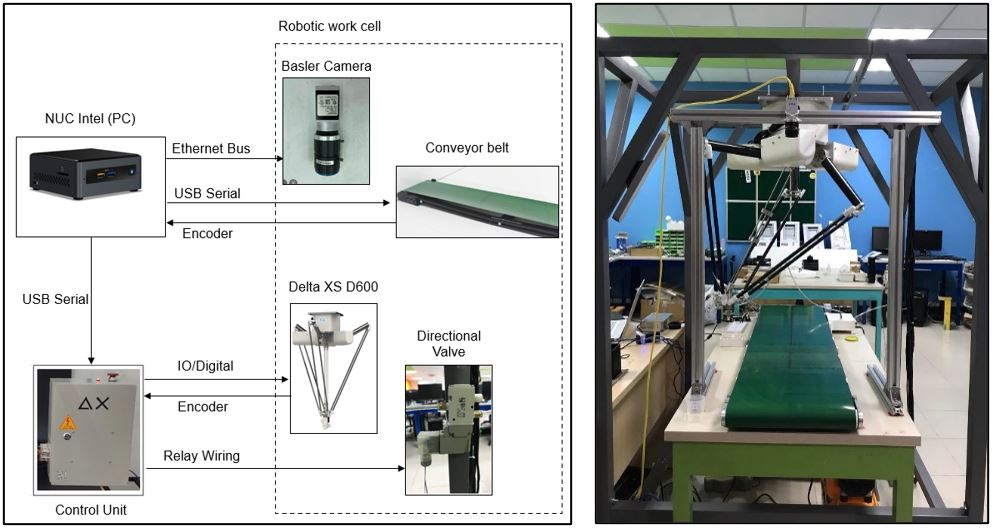
\includegraphics[width=0.9\textwidth]{fig15.JPG}
        \caption{Schematic (left) \& Actual (right) setups of robot work cell }
    \end{figure}
    The Delta XS D600 robot is mounted to the iron frame in which the four legs are fixed to the floor to reduce vibration and movement of the frame. Moreover, the conveyor is set up under the robot so that the central line along the conveyor has to be aligned with the Y axis of the robot coordination. This helps defining the coordinates of the nuts and implementing the pick and place algorithm further on. In addition, the object detection system is applied to detect the defected nuts moving on the conveyor belt. The camera is positioned perpendicular to the conveyor surface and 560 mm far away from the original point of the robot (right after the loading area) to detect the coordinates of the nut on the horizontal surface.\par
    \begin{figure}[h]
        \centering
        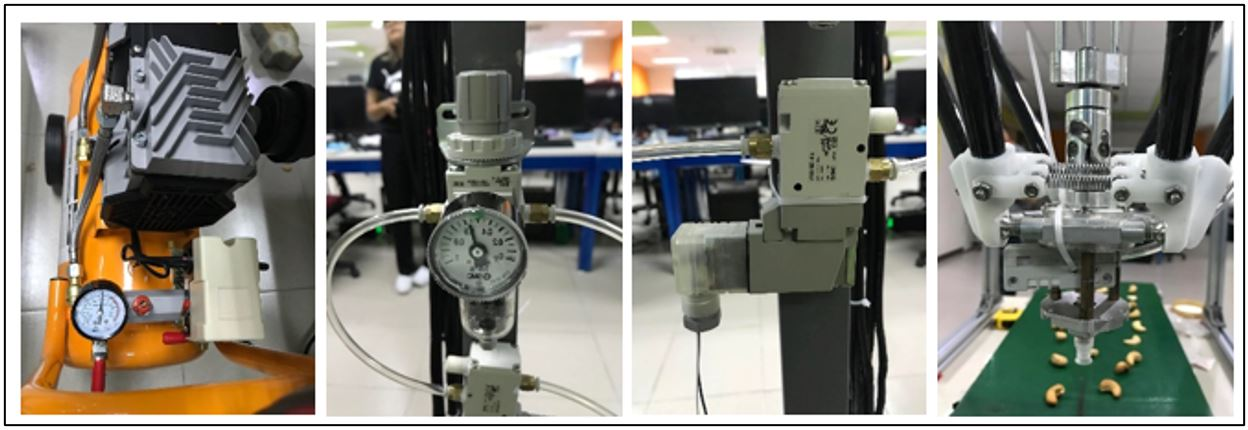
\includegraphics[width=\textwidth]{fig16.JPG}
        \caption{Pneumatic system setup}
    \end{figure}
    To prevent the vibration of the camera, it is placed on its separated frame instead of hanging on the robot frame. Since the robot, the camera, and the conveyor have to be synchronized, for this purpose, the reference frame is presented with their transformation matrices in the following cashew nuts picking strategy section. \par
    For vacuuming of the nuts, the pneumatic system is set up separately. Initially, the air compressor is placed under the conveyor and fresh air area to ensure that it is not heated during operation time. Then, the FR Unit is placed on the robot frame and faces the operation table to conveniently monitor and adjust the air pressure. The directional control valve is set up right after the FR Unit and close to the Control Unit of the robot arm so that the controller box of the robot also controls the directional valve as using PLC. Finally, the ejector is placed at the end effector of the robot to create the vacuum feature to pick up the defected nuts. \par

\subsection{Communication between camera system and robotic system}
    \begin{figure}[h]
        \centering
        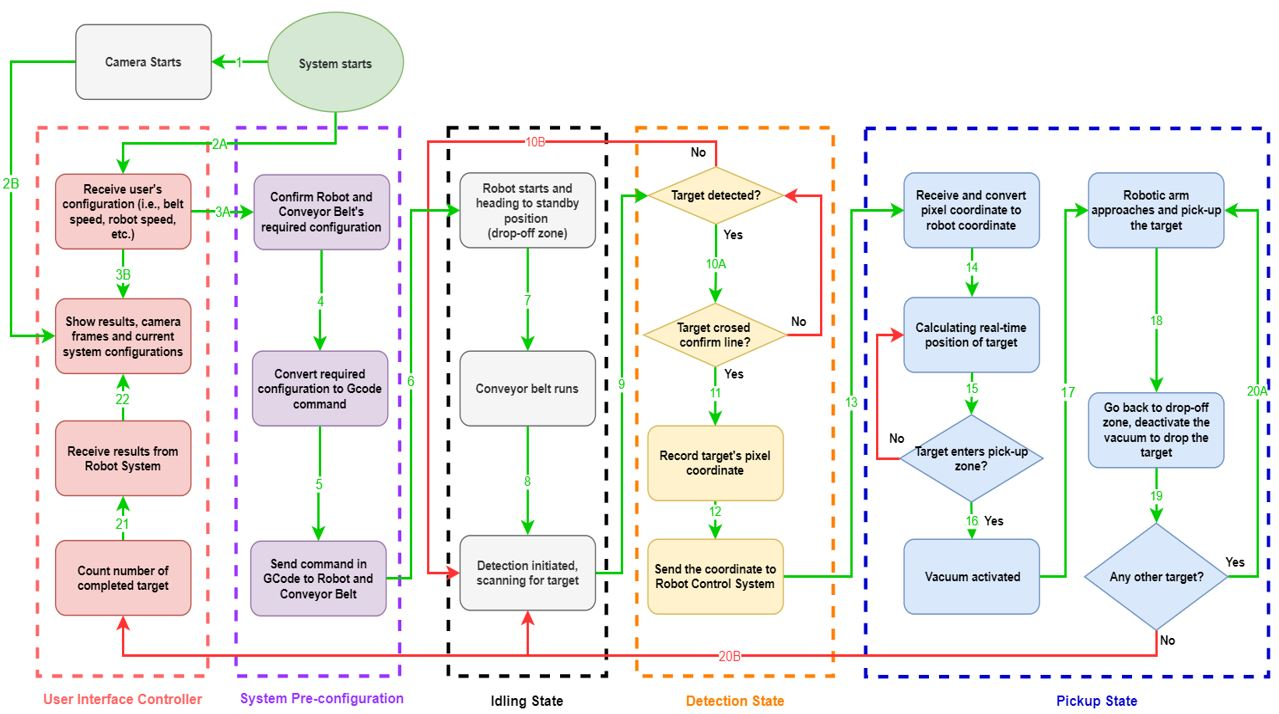
\includegraphics[width=\textwidth]{fig17.JPG}
        \caption{Diagram of the complete system}
    \end{figure}
    The diagram above (figure 17) illustrates the connection between each module in form of different states. As the system is initiated, the camera will be activated and starts providing real-time streaming frames. Then, the pre-defined configuration will be converted into G-code, and applied immediately to the hardware at the System Pre-configuration state. \par
    When the configuration has been successfully implemented, all hardware modules are set in motion. Firstly, the robot arm will be sent home to ensure the proper working of all axis, before arriving at the standby position, in which the defected cashew nuts are dropped-off. Concurrently, the conveyor belt starts to run at a determined speed to carry each batch of cashew nuts going past the camera module, with the detection algorithm commencing. This process occurs at the Detection State, in which the target will be recognized and tracked. When a confirmed target passes through the confirmation border, its coordinate will be recorded and sent to the Robotics System. \par
    \begin{figure}[h]
        \centering
        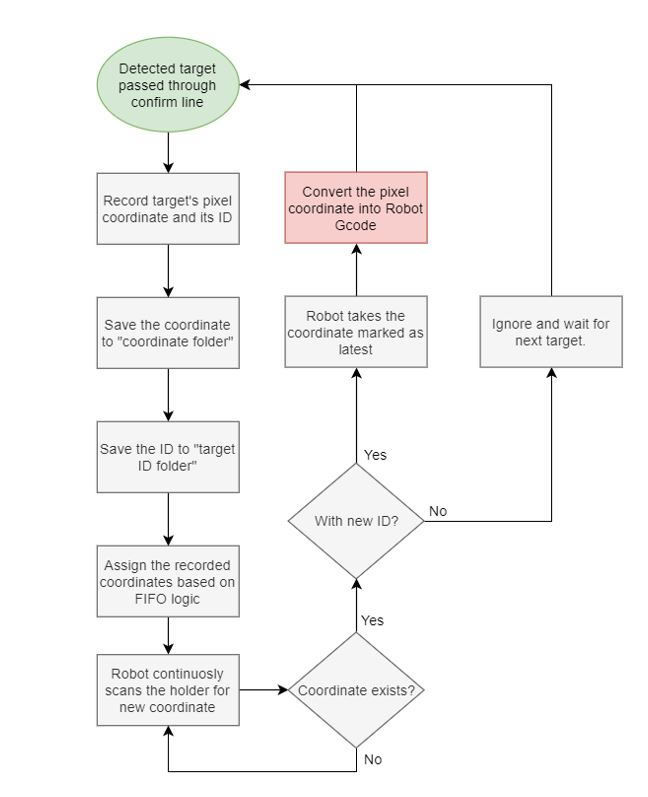
\includegraphics[width=0.7\textwidth]{fig18.JPG}
        \caption{Coordinate sending between camera and robot}
    \end{figure}
    Receiving the pixel coordinate of the target, the robotic processor performs various tasks to convert the pixel coordinate into a robotic coordinate. When the target reaches the robot’s working radius, the vacuum will be activated, and the robot arm will immediately approach the target and pick it up, then the robot will move back to the drop-off point and drop the object by deactivating the vacuum. The same process consecutively applies to other targets. \par
    When a defected nut reaches the confirmation line marked on the camera frame, its current coordinate and ID are recorded and stored in a separate folder. When multiple objects pass the line concurrently, the coordinates will be assigned in a First-In-First-Out (FIFO) order. The robot system will automatically scan the folder to see if any object has been recorded. When a coordinate exists, the object ID will then be compared to see whether that coordinate has been processed previously. If it is a new ID, the robot will take that coordinate and convert it for G-code. Otherwise, the coordinate will be discarded. Utilizing a unique Object ID for an individual object would help prevent an object’s coordinate from being sent infinitely after crossing the confirmation line. \par
    \begin{figure}[h]
        \centering
        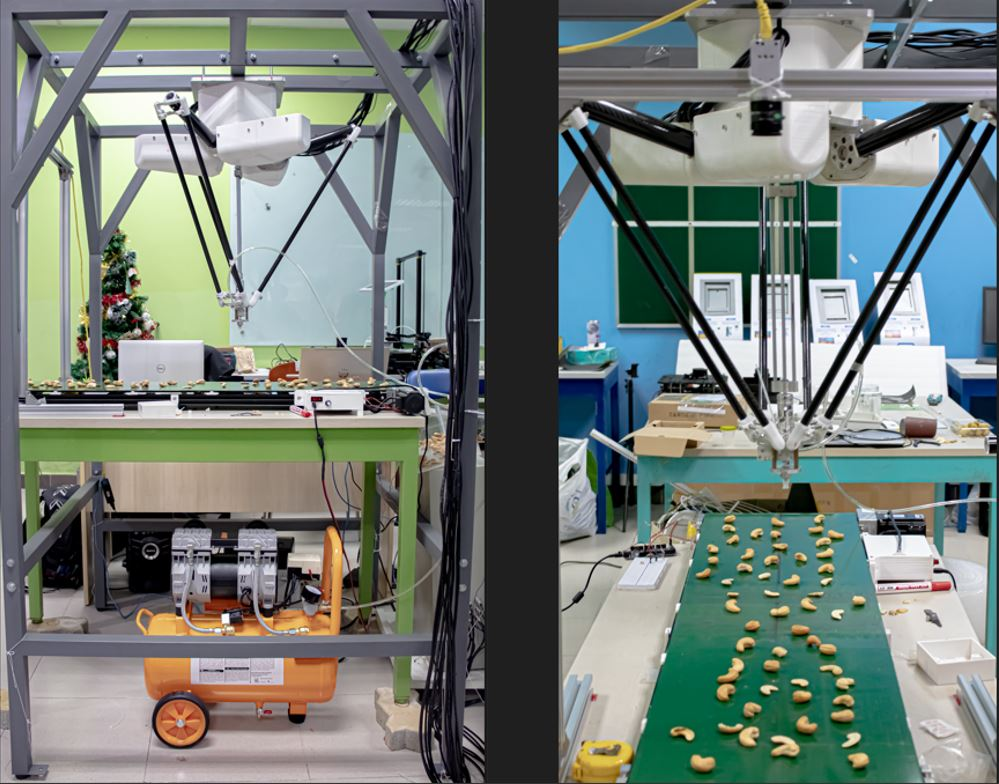
\includegraphics[width=0.8\textwidth]{fig19.JPG}
        \caption{Picture of completed system}
    \end{figure}

\section{EXPERIMENTAL RESULTS AND DISCUSSION}

\subsection{Model evaluation and detection accuracy of faulted cashew nuts}
    \begin{table}[h!]
        \centering
        \renewcommand{\arraystretch}{1.5}
        \setlength{\tabcolsep}{11pt}
        \caption{Evaluation of models}\label{table2}
        \begin{tabular}{ccccc}
            % { m{3cm} m{1.7cm} m{1.7cm} m{1.7cm} m{1.7cm} } 
            \hline 
            Model & Precision & Recall & F1-score & mAP\@0.50 \\ 
            \hline 
            YOLOv4-tiny-416 & 97.66\% & 97.09\% & 97.38\% & 97.66\%\\
            YOLOv4-tiny-608 & \textbf{98.82\%} & \textbf{97.67\%} & \textbf{98.25\%} & \textbf{98.35\%}\\ 
            YOLOv4-tiny-800 & 98.23\% & 97.09\% & 97.66\% & 98.17\%\\
            \hline
        \end{tabular}
    \end{table}
    After 3,000 iterations, the training process is finished when no significant improvements have been observed in the average loss. In contrast, further training would result in over-fitting the model. Appendix 4 shows the chart of average loss versus iterations number of YOLOv4-tiny-608, along with the mAP percentage of each iteration after the loss had greatly decreased. Based on the number of true positives, false positives, and false negatives of each model, we calculated the precision, recall, F1-score, and mAP at intersection over union of 50\%.\par 
    Table 2 shows the scores of three YOLOv4-tiny models, trained with 416x416, 608x608, and 800x800 image resolutions. Out of the three models, YOLOv4-tiny-608 gave the highest score in all parameters, with 98.82\% precision, 97.67\% recall, 98.25\% F1-score, and 98.35\% mAP@0.50. Testing with new images, 416 x 416 resolution has the lowest accuracy, while 608 x 608 and 800 x 800 models output higher accuracies (Figure 20). Nevertheless, in both test set and the newly acquired test images, YOLOv4-tiny-608 still results in the highest accuracy.\par
    \begin{figure}[h]
        \centering
        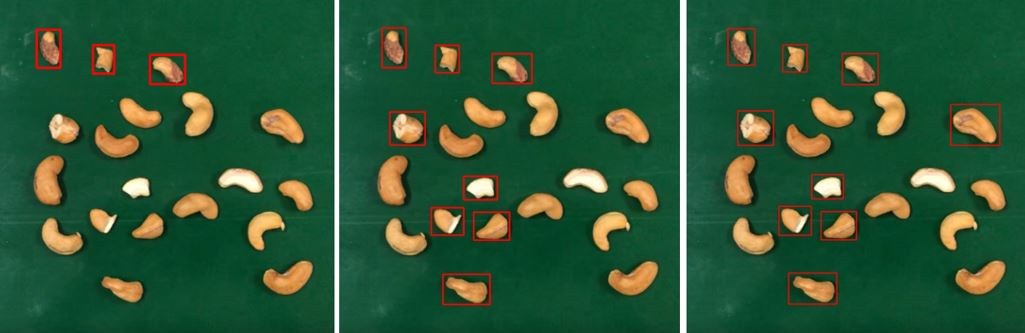
\includegraphics[width=\textwidth]{fig21.JPG}
        \caption{Detection of YOLOv4-tiny: 416x416 (left), 608x608 (middle), 800x800 (right)}
    \end{figure}

\subsection{Pick-and-place accuracy of faulted cashew nuts}

\subsubsection*{The efficiency of suction cups}
    \begin{figure}[h]
        \centering
        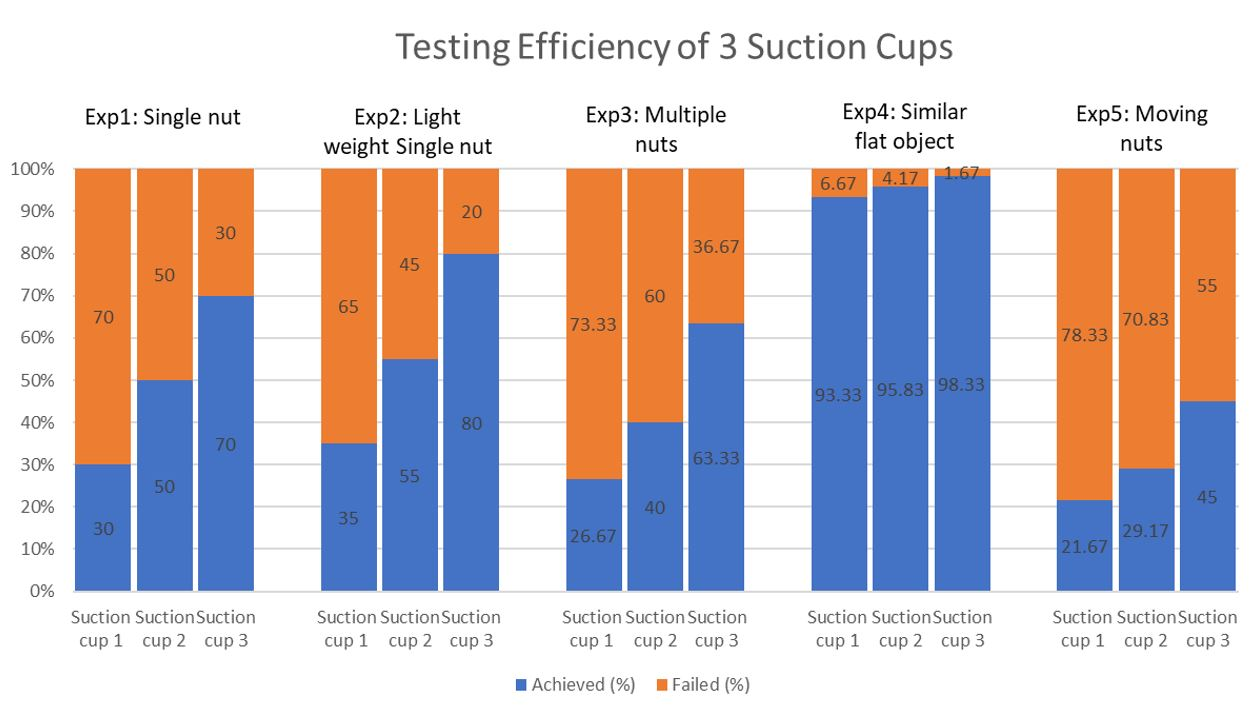
\includegraphics[width=0.9\textwidth]{fig22.JPG}
        \caption{Results of 5 experiments testing the efficiency of 3 suction cups}
    \end{figure}
    The purpose of these 5 experiments is to illustrate the results of efficiency in picking cashew nuts for three different types of suction cups. There are five experiments including picking single nuts and multiple nuts, picking similar flat objects in the static condition, and picking multiple nuts in moving condition. Moreover, the maximum pressure and power of the air supply for these experiments are 0.7MPa, and 3/4 HP respectively. The results are shown in Figure 21.\par
    Experiment 1 concludes that the more stages in the shape of the suction cup, the more efficient it is in picking the cashew nut. Besides, experiment 2 shows that increasing the pressure of supplied air source can improve the quality of picking nuts. Then, by experimenting 3 we can conclude that the varieties of nut orientation, the surface, and even the height can affect the quality and efficiency of the picking task. The results from experiment 4 strongly conclude again that the varieties of nut orientation, the surface, and even the height significantly affect the quality and efficiency of the picking task. Finally, experiment 5 shows that the efficiency in picking nuts of all the suction cups is low with the moving nuts having different orientations, surface, and height. In summary, Suction cup 3 is the most suitable candidate for this application.\par

\subsubsection*{The efficiency of the position prediction algorithm}
    The proposed picking position prediction algorithm has been intensively tested in the picking process. Several tests with the varieties of conveyor speeds were performed and the robot end effector approached each single target nut successfully and accurately. The results of testing the accuracy of the algorithm are shown in table 3\par
    \begin{table}[h!]
        \caption{Position and repetition accuracies of the algorithm according to a variety of conveyor speed}\label{table3}
        \centering
        \renewcommand{\arraystretch}{1.75}
        \setlength{\tabcolsep}{7pt}
        \begin{tabular}{ ccccccc }
        \hline
        \multirow{2}{1.5cm}{Speed of conveyor belt}  &
        \multicolumn{2}{c}{Left error (mm)} &
        \multicolumn{2}{c}{Middle error (mm)} &
        \multicolumn{2}{c}{Right error (mm)}\\ 
        \cline{2-7}
        & X-axis & Y-axis & X-axis & Y-axis & X-axis & Y-axis\\
        \hline
        15 mm/s & 0 & 0.08 - 0.15 & 0 & 0.05 - 0.08 & 0 & 0.06\\
        25 mm/s & 0 & 0.19 – 0.22 & 0 & 0.20 & 0 & 0.20\\
        35 mm/s & 0 & 0.20 – 0.27 & 0 & 0.27 & 0 & 0.27\\
        \hline
        \end{tabular}
    \end{table}
    The position accuracy of the algorithm is slightly increased by approximately 0.15 mm when increasing the speed of the conveyor belt with the step of 5 mm/s. In details, as increasing the speed of the conveyor, the actual position of the nut is changed faster than the updated result of the nut position in the computer. This is because the configuration of the NUC Intel chip cannot handle both the robotic system and computer vision system at the same time which causes a delay to the position value in the computer compared to the actual ones. An upgrade to the computer hardware would improve the performance of the pick-and-place operation, so that the CPU can handle multiple tasks at a higher speed.\par

\section{CONCLUSION AND FUTURE STUDIES}
    In this paper, we have discussed the necessity of an automated solution for cashew sorting in the final quality checking stage of a cashew nuts production line. In order to cope with the shortage of skilled workers, a system was developed to detect faulted cashew nuts in a kernel, then pick and place them outside of the working area, by applying computer vision, robotic manipulator, and pneumatic system.\par
    For the machine vision system, we have collected a dataset of 1,500 standard and faulted cashew nuts, and performed transfer learning through the pre-trained YOLOv4-tiny model, in order to recognize the presence of multiple defected nuts in a deshelled cashew kernel. Out of the three input image resolutions (406 x 406, 608 x 608, 800 x 800), the YOLOv4-tiny-608 model gave the highest accuracy of 98.35\%. Then, the real-time detection was processed along with camera calibration to track and transform pixel coordinates of the targets into world coordinates for the pick-and-place operation.\par 
    For the robotics system, firstly, we have discussed the working and controlling mechanism of Delta XS D800 parallel robot, which is controlled by sending G-Code from PC through the Teensy Duino MCU using UART transmission. With the help of the pneumatic system, the robot arm was able to pick and place the detected nuts outside of the working area, using a suction cup as the end effector. Through several static and dynamic tests with three different suction cups, the cup outputs the highest accuracy was selected.\par
    Finally, regarding the integration of machine vision and robotics modules, the reference frame and frame transformation were chosen and performed to be compatible with the system setup. Moreover, the First-In-First-Out (FIFO) picking strategy was also mentioned to remove the nuts in an order. After testing with different conveyor belt speeds, it is noted that the position error is increased by 0.15 mm when increasing the speed by 5 mm/s, due to the limited computational power of the NUC Intel chip when integrating both computer vision and robotics modules together.\par
    In future studies, an upgrade to hardware can offer a better result to the overall system, such as a more powerful CPU, or equipped with a GPU to handle both object detection and robot pick-and-place tasks faster and more efficiently. Furthermore, regard to the picking accuracy of the suction cup, an alternative solution such as a cyclone vacuum can be considered to increase the performance of the removal process.\par

\subsubsection*{Acknowledgement}
    This paper presents a part of the research project sponsored by TMA Innovation in collaboration with the School of Science, Engineering, and Technology (SSET), RMIT Vietnam. Other members contributing to the project include Trieu Hoang, Minh Nguyen Tran, Khoi Vu from RMIT University and Thang Tran, Chau Nguyen from TMA Innovation.

\pagebreak
\section*{Appendix 1}
    \begin{table}[h!]
        \caption*{YOLOv4-tiny-416 network configuration}
        \centering
        \renewcommand{\arraystretch}{1}
        \begin{tabular}{c c c c c c}
            \hline
            Layer & Type & Filters & Size/Stride & Input & Output \\ 
            \hline
            0 & Convolutional & 32 & 3 x 3/ 2 & 416 x 416 x 3 & 208 x 208 x 32 \\
            1 & Convolutional & 64 & 3 x 3/ 2 & 208 x 208 x 32 & 104 x 104 x 64  \\
            2 & Convolutional & 64 & 3 x 3/ 1 & 104 x 104 x 64 & 104 x 104 x 64\\
            3 & Route 2				\\
            4 & Convolutional & 32 & 3 x 3/ 1 & 104 x 104 x 32 & 104 x 104 x 32\\
            5 & Convolutional & 32 & 3 x 3/ 1 & 104 x 104 x 32 & 104 x 104 x 32\\
            6 & Route 5 4				\\
            7 & Convolutional & 64 & 1 x 1/ 1 & 104 x 104 x 64 & 104 x 104 x 64\\
            8 & Route 2 7				\\
            9 & Maxpool & {} & 2 x 2/ 2 & 104 x 104 x 128 & 52 x 52 x 128\\
            10 & Convolutional & 128 & 3 x 3/ 1 & 52 x 52 x 128 & 52 x 52 x 128\\
            11 & Route 10				\\
            12 & Convolutional & 64 & 3 x 3/ 1 & 52 x 52 x 64 & 52 x 52 x 64\\
            13 & Convolutional & 64 & 3 x 3/ 1 & 52 x 52 x 64 & 52 x 52 x 64\\
            14 & Route 13 12				\\
            15 & Convolutional & 128 & 1 x 1/ 1 & 52 x 52 x 128 & 52 x 52 x 128\\
            16 & Route 10 15				\\
            17 & Maxpool & {} & 2 x 2/ 2 & 52 x 52 x 256 & 26 x 26 x 256\\
            18 & Convolutional & 256 & 3 x 3/ 1 & 26 x 26 x 256 & 26 x 26 x 256\\
            19 & Route 18				\\
            20 & Convolutional & 128 & 3 x 3/ 1 & 26 x 26 x 128 & 26 x 26 x 128\\
            21 & Convolutional & 128 & 3 x 3/ 1 & 26 x 26 x 128 & 26 x 26 x 128\\
            22 & Route 21 20				\\
            23 & Convolutional & 256 & 1 x 1/ 1 & 26 x 26 x 256 & 26 x 26 x 256\\
            24 & Route 18 23				\\
            25 & Maxpool & {} & 2 x 2/ 2 & 26 x 26 x 512 & 13 x 13 x 512\\
            26 & Convolutional & 512 & 3 x 3/ 1 & 13 x 13 x 512 & 13 x 13 x 512\\
            27 & Convolutional & 256 & 1 x 1/ 1 & 13 x 13 x 512 & 13 x 13 x 256\\
            28 & Convolutional & 512 & 3 x 3/ 1 & 13 x 13 x 256 & 13 x 13 x 512\\
            29 & Convolutional & 21 & 1 x 1/ 1 & 13 x 13 x 512 & 13 x 13 x 21\\
            30 & YOLO				\\
            31 & Route 27				\\
            32 & Convolutional & 128 & 1 x 1/ 1 & 13 x 13 x 256 & 13 x 13 x 128\\
            33 & Upsample & {} & 2 x 2/1 & 13 x 13 x 128 & 26 x 26 x 128\\
            34 & Route 33 23				\\
            35 & Convolutional & 256 & 3 x 3/ 1 & 26 x 26 x 384 & 26 x 26 x 256\\
            36 & Convolutional & 21 & 1 x 1/ 1 & 26 x 26 x 256 & 26 x 26 x 21\\
            37 & YOLO				\\
            \hline
        \end{tabular}
    \end{table}  

\section*{Appendix 2}
    \begin{figure}[h]
        \centering
        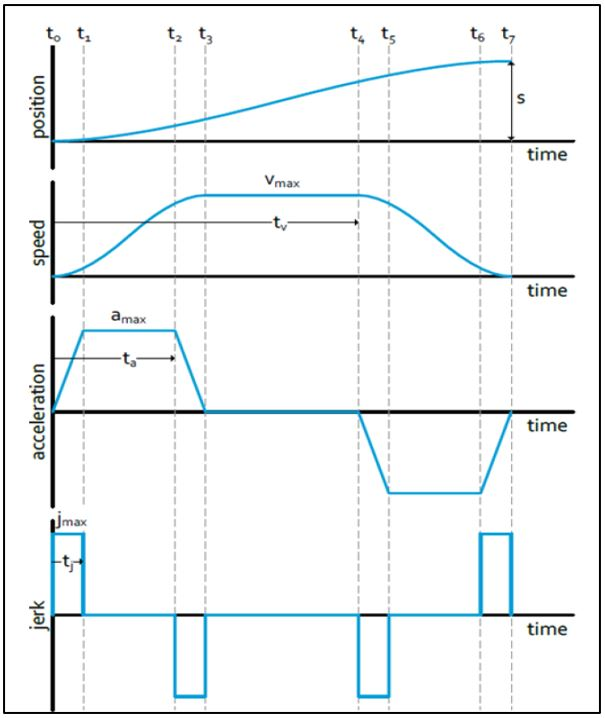
\includegraphics[width=0.6\textwidth]{appendix2.JPG}
        \caption*{S-curve profile}
    \end{figure}

\section*{Appendix 3}
    \begin{figure}[h]
        \centering
        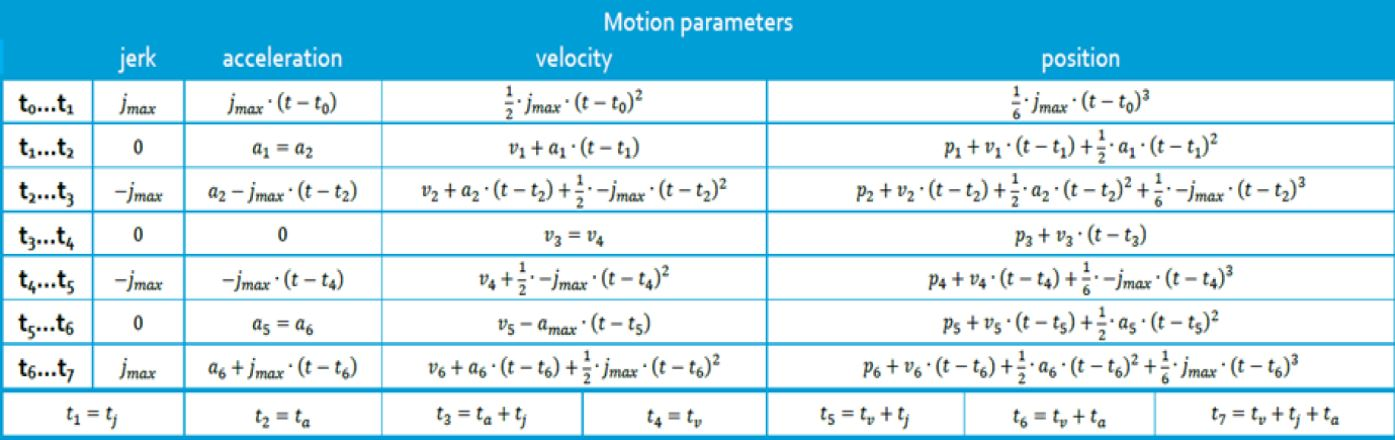
\includegraphics[width=\textwidth]{appendix3.JPG}
        \caption*{S-curve motion parameters portfolio}
    \end{figure}
\pagebreak
\section*{Appendix 4}
    \begin{figure}[h]
        \centering
        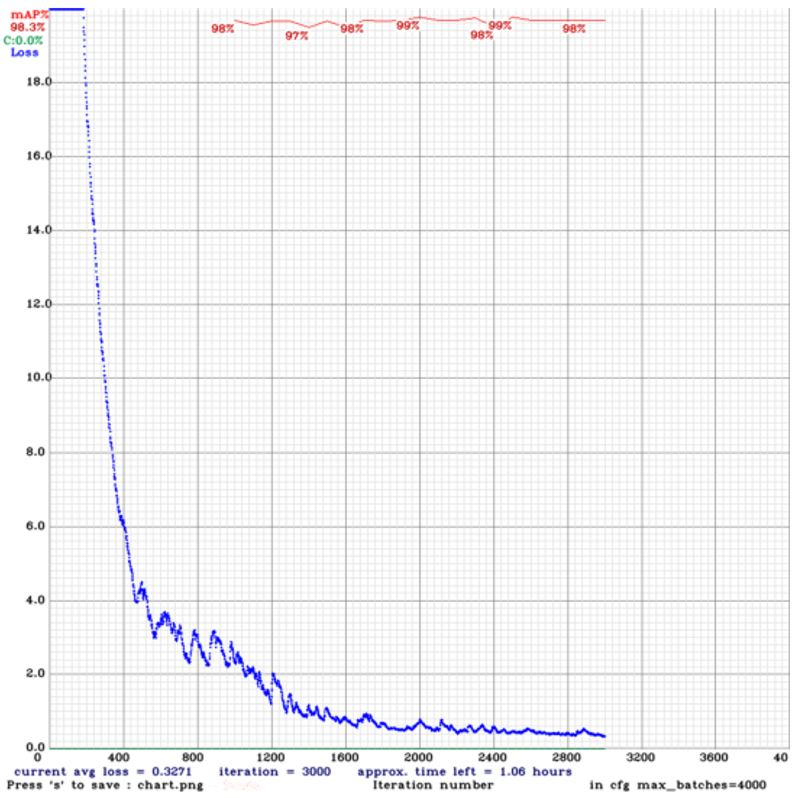
\includegraphics[width=\textwidth]{fig20.JPG}
        \caption*{Training result of YOLOv4-tiny-608}
    \end{figure}

\pagebreak
\section*{REFERENCES}
    \begin{enumerate}
        \item N. N. Oliveira, C. G. Mothé, M. G. Mothé, and L. G. de Oliveira, "Cashew nut and cashew apple: a scientific and technological monitoring worldwide review," Journal of Food Science and Technology, vol. 57, no. 1, pp. 12-21, 2020.
        \item O. Kilanko, "Design and performance evaluation of centrifugal cashew nut sheller," Agricultural Engineering International: CIGR Journal, vol. 20, no. 1, pp. 162-170, 2018.
        \item A. Singh, V. Aware, P. Shahare, S. Sonawane, K. Dhande, and S. Aware, "Development of Power Operated Cashew Nut Deshelling Machine," Journal of Ready to Eat Food| July-September, vol. 7, no. 03, pp. 31-38, 2020.
        \item J. Du, "Understanding of object detection based on CNN family and YOLO," in Journal of Physics: Conference Series, 2018, vol. 1004, no. 1: IOP Publishing, p. 012029.
        \item R. Huang, J. Pedoeem, and C. Chen, "YOLO-LITE: A Real-Time Object Detection Algorithm Optimized for Non-GPU Computers," IEEE International Conference on Big Data, 2018.
        \item M. Dong et al., "State of the art in parallel ankle rehabilitation robot: a systematic review," Journal of NeuroEngineering and Rehabilitation, vol. 18, no. 1, pp. 1-15, 2021.
        \item S. Lilge, K. Nuelle, G. Boettcher, S. Spindeldreier, and J. Burgner-Kahrs, "Tendon actuated continuous structures in planar parallel robots: A kinematic analysis," Journal of Mechanisms and Robotics, vol. 13, no. 1, 2021.
        \item A. Lohia, K. D. Kadam, R. R. Joshi, A. M. Bongale, and M. Anupkumar, "Bibliometric Analysis of One-stage and Two-stage Object Detection," Libr. Philos. Pract, vol. 4910, 2021.
        \item A. Bochkovskiy, C.-Y. Wang, and H.-Y. M. Liao, "Yolov4: Optimal speed and accuracy of object detection," arXiv preprint arXiv:2004.10934, 2020.
        \item C.-Y. Wang, H.-Y. M. Liao, Y.-H. Wu, P.-Y. Chen, J.-W. Hsieh, and I.-H. Yeh, "CSPNet: A new backbone that can enhance learning capability of CNN," in Proceedings of the IEEE/CVF conference on computer vision and pattern recognition workshops, 2020, pp. 390-391. 
        \item S. Liu, L. Qi, H. Qin, J. Shi, and J. Jia, "Path aggregation network for instance segmentation," in Proceedings of the IEEE conference on computer vision and pattern recognition, 2018, pp. 8759-8768. 
        \item F. J. P. Montalbo, "A computer-aided diagnosis of brain tumors using a fine-tuned YOLO-based model with transfer learning," KSII Transactions on Internet and Information Systems (TIIS), vol. 14, no. 12, pp. 4816-4834, 2020.
        \item H. C. Bazame, J. P. Molin, D. Althoff, and M. Martello, "Detection, classification, and mapping of coffee fruits during harvest with computer vision," Computers and Electronics in Agriculture, vol. 183, p. 106066, 2021.
        \item T.-Y. Lin et al., "Microsoft coco: Common objects in context," in European conference on computer vision, 2014: Springer, pp. 740-755. 
        \item V. Mazzia, A. Khaliq, F. Salvetti, and M. Chiaberge, "Real-time apple detection system using embedded systems with hardware accelerators: An edge AI application," IEEE Access, vol. 8, pp. 9102-9114, 2020.
        \item M. Wilson, The Implementation of Robot Systems, 2nd ed. Butterworth-Heinemann, 2015, pp. 19-38.
        \item A. Kurniawan, Teensy Development Workshop, 1st ed. Depok, 2015, pp. 5-6.
        \item S. G. Zain and N. Nirwana, "Prototipe Antena Tracker Menggunakan Motor Stepper Nema 23 sebagai Aktuator 2 Axis," in Seminar Nasional LP2M UNM, 2019. 
        \item I. Ioana, M. Blejan and R. Blejan, "S-curve motion profiles generator for hydraulic actuators", 2019. 
    \end{enumerate}

\end{document}